% example.tex -- A sample LaTeX code
\documentclass{article}
\usepackage{amsmath}
\usepackage{graphicx}

\title{Exercise 1}
\author{Eric Fernando}
\date{\today}

\begin{document}

\maketitle

\section{What does an engineering student do when he has too much time?}
He listens to Bob Marley.

\subsection{An equation}

\begin{equation}
plot(\theta) = (1+0.9*cos(8*\theta))(1+0.1*cos(24*\theta))(0.9+0.05*cos(200*\theta))(1+sin(\theta))
\end{equation}


\subsection{The plot}


\begin{figure}[h]
  \caption{Equation plotted in polar axes.}
  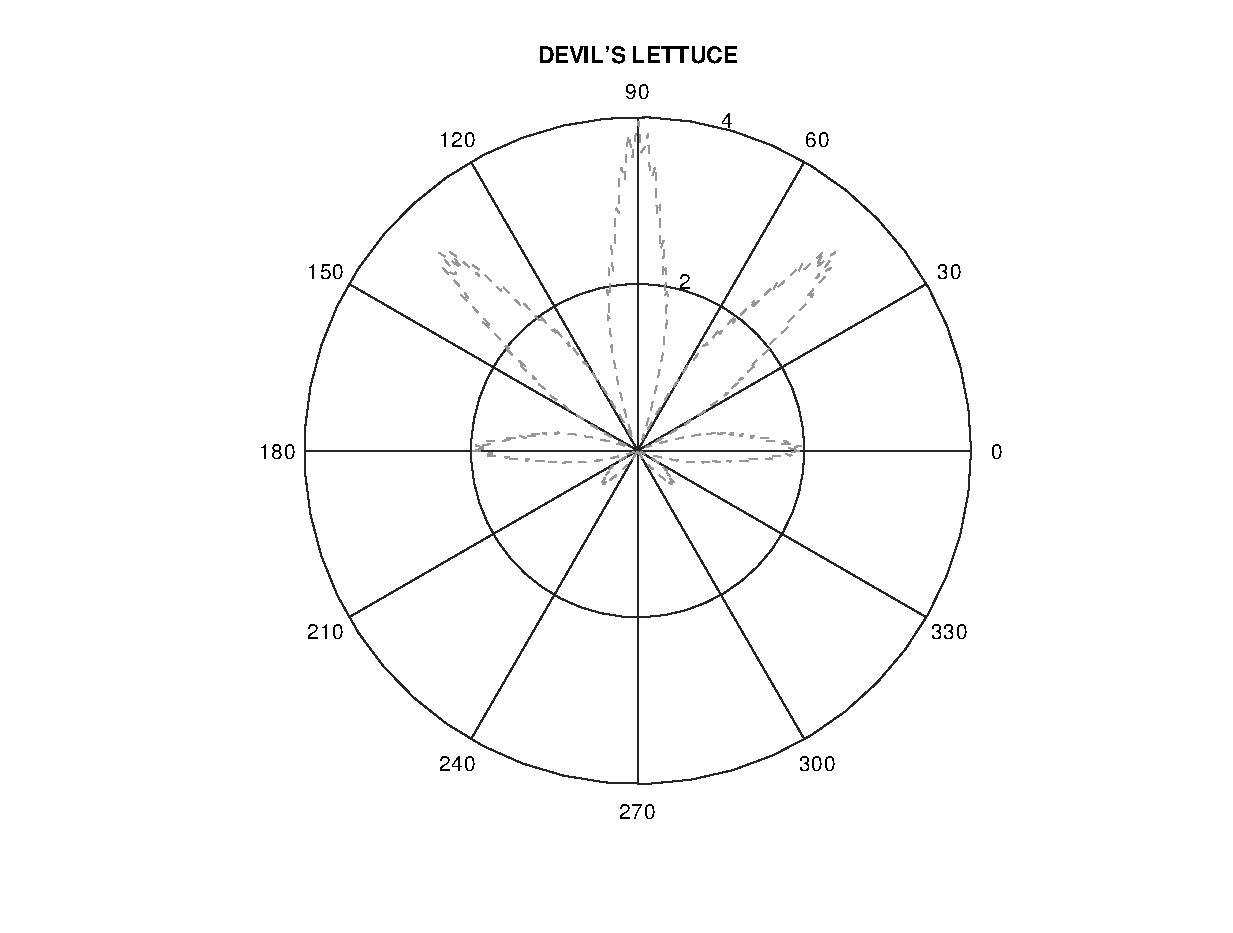
\includegraphics[width=0.9\textwidth]{img.eps}

\end{figure}

\subsection{All the Bob Marley Songs I listened to today}

\begin{table}[h]
  \centering
    \begin{tabular}{| l c r |}
    \hline
    1 & Is This Love & 3:52\\
    2 & No Woman, No Cry & 4:05\\
    3 & Could You Be Loved & 3:33\\
    4 & Exodus & 5:24\\
    5 & Jamming & 3:17\\	
    \hline
    \end{tabular}
  \caption{Bob Marley songs}
\end{table}

\end{document}
